%%%%%%%%%%%%%%%%%%%%%%%%%%%%%%%%%%%%%%%%%
% Beamer Presentation
% LaTeX Template
% Version 1.0 (10/11/12)
%
% This template has been downloaded from:
% http://www.LaTeXTemplates.com
%
% License:
% CC BY-NC-SA 3.0 (http://creativecommons.org/licenses/by-nc-sa/3.0/)
%
%%%%%%%%%%%%%%%%%%%%%%%%%%%%%%%%%%%%%%%%%

%----------------------------------------------------------------------------------------
%	PACKAGES AND THEMES
%----------------------------------------------------------------------------------------

\documentclass[14pt,handout]{beamer}
%%\documentclass[14pt]{beamer}

\mode<presentation> {

% The Beamer class slide themes
\usetheme{Madrid} %i was using this one

% Beamer class color themes

%\usecolortheme{albatross}

%\setbeamertemplate{footline} % To remove the footer line in all slides uncomment this line
%\setbeamertemplate{footline}[page number] % To replace the footer line in all slides with a simple slide count uncomment this line

%\setbeamertemplate{navigation symbols}{} % To remove the navigation symbols from the bottom of all slides uncomment this line
}

\usepackage{graphicx} % Allows including images
\usepackage{booktabs} % Allows the use of \toprule, \midrule and \bottomrule in tables
\usepackage{hyperref}
\usepackage{helvet}
\usepackage[T1]{fontenc}
\usepackage{textcomp}

%----------------------------------------------------------------------------------------
%	TITLE PAGE
%----------------------------------------------------------------------------------------

\title[RNAseq Practical pt2/3]{RNAseq Walkthrough (now with Genes \& Geography)} % The short title appears at the bottom of every slide, the full title is only on the title page

\author{C. Ryan Campbell} % Your name
\institute[Duke] % Your institution as it will appear on the bottom of every slide, may be shorthand to save space
{
Duke University \\ % Your institution for the title page
\medskip
\textit{c.ryan.campbell@duke.edu} % Your email address
}
\date{2 Nov 2017} % Date, can be changed to a custom date

\begin{document}

\begin{frame}
\titlepage % Print the title page as the first slide
\end{frame}

\begin{frame}
\frametitle{Overview} % Table of contents slide, comment this block out to remove it
\tableofcontents % Throughout your presentation, if you choose to use \section{} and \subsection{} commands, these will automatically be printed on this slide as an overview of your presentation
\end{frame}

%----------------------------------------------------------------------------------------
%	PRESENTATION SLIDES
%----------------------------------------------------------------------------------------

%------------------------------------------------
\begin{frame}
\frametitle{Today's Goals}
\begin{itemize}
	\item<+-> Run tophat2
	\item<+-> Run htseq-count
	\item<+-> Understand htseq-count output
\end{itemize}
\end{frame}

%------------------------------------------------
\section{Genes \& Geography}
%------------------------------------------------

%------------------------------------------------
\begin{frame}
\frametitle{Lessa 1990}
\begin{center}
		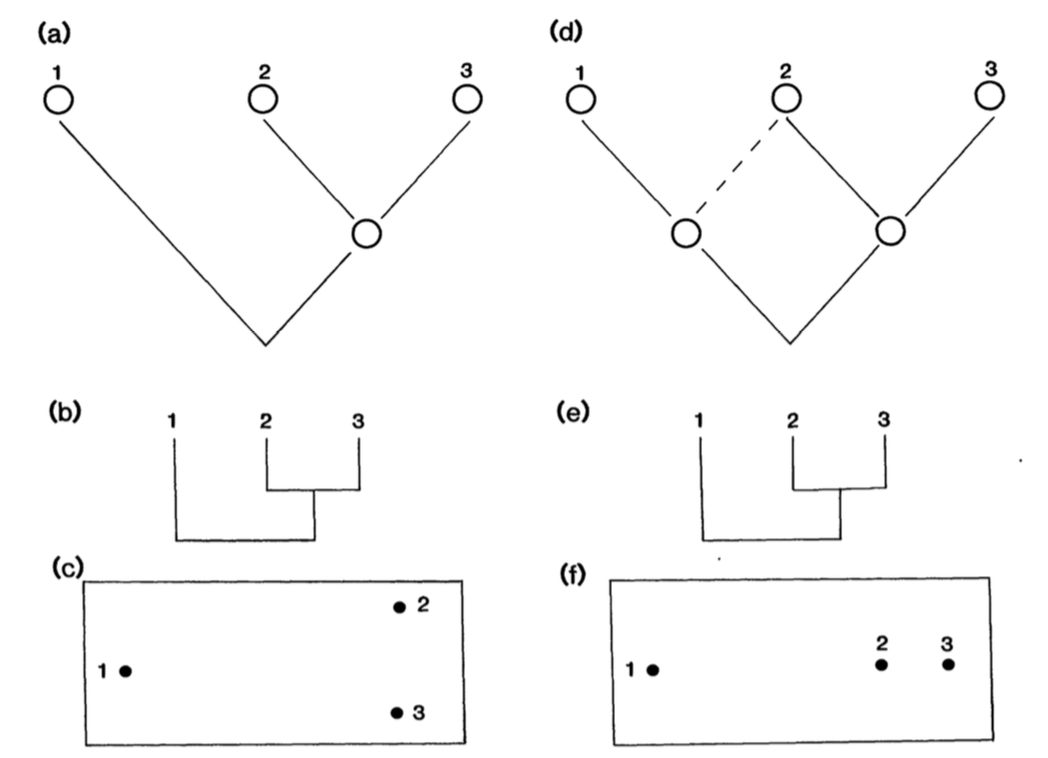
\includegraphics[width=.9\textwidth]{images_20171102_gg01.png}
\end{center}
\end{frame}

%------------------------------------------------
\begin{frame}
\frametitle{Lessa 1990}
\begin{center}
		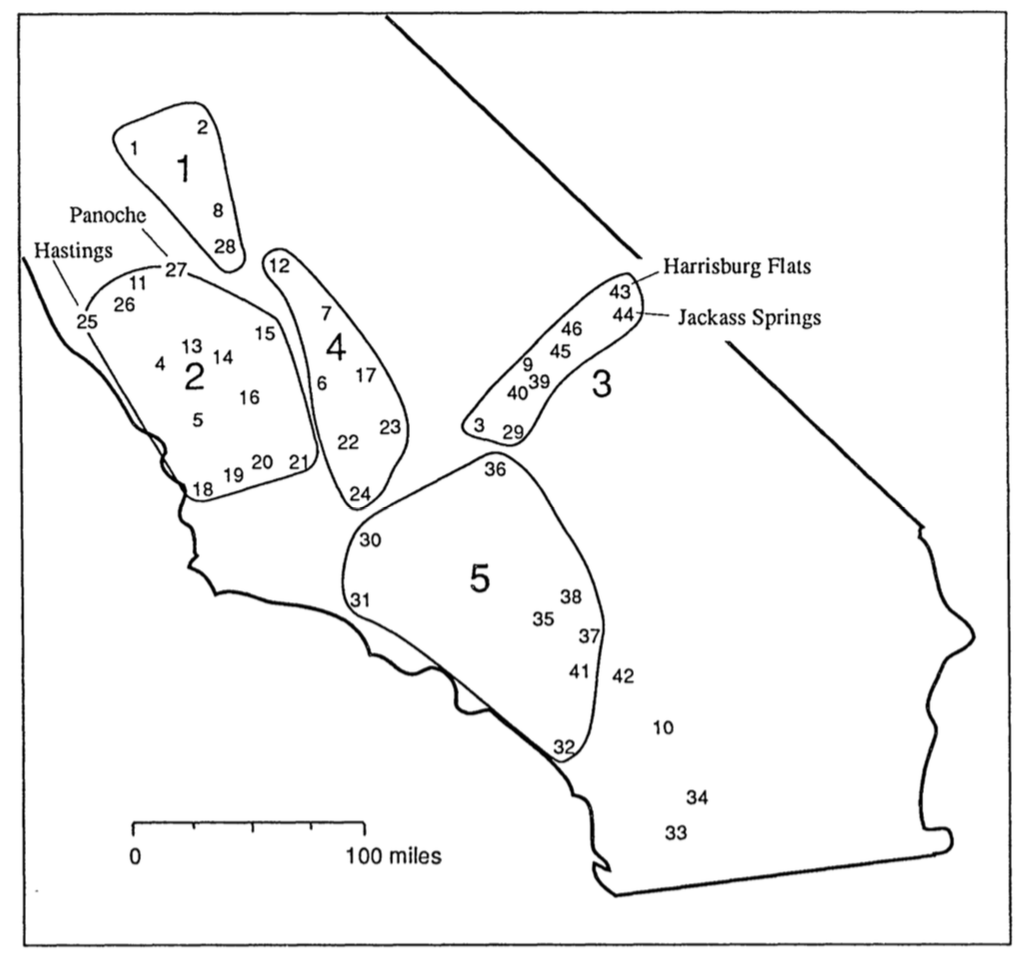
\includegraphics[width=.7\textwidth]{images_20171102_gg02.png}
\end{center}
\end{frame}

%------------------------------------------------
\begin{frame}
\frametitle{Lessa 1990}
\begin{center}
		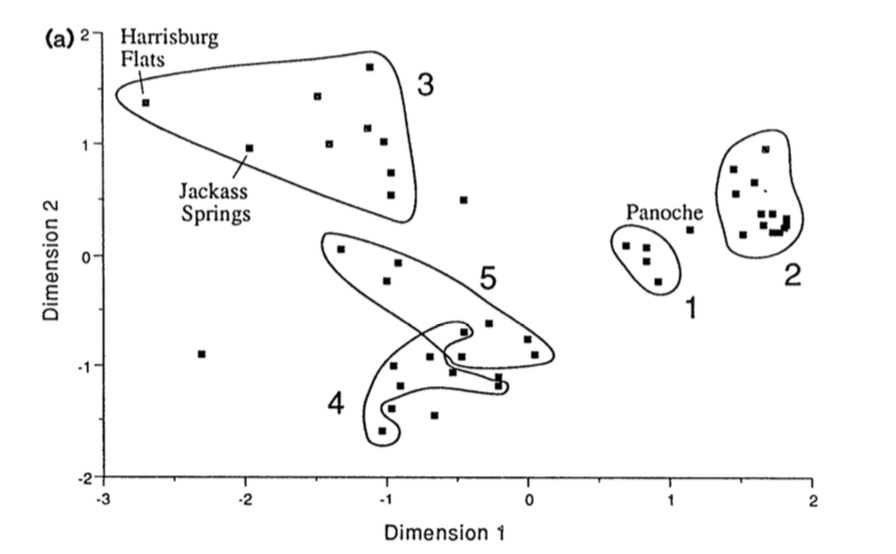
\includegraphics[width=.9\textwidth]{images_20171102_gg03.png}
\end{center}
\end{frame}

%------------------------------------------------
\begin{frame}
\frametitle{Novembre 2008}
\begin{center}
		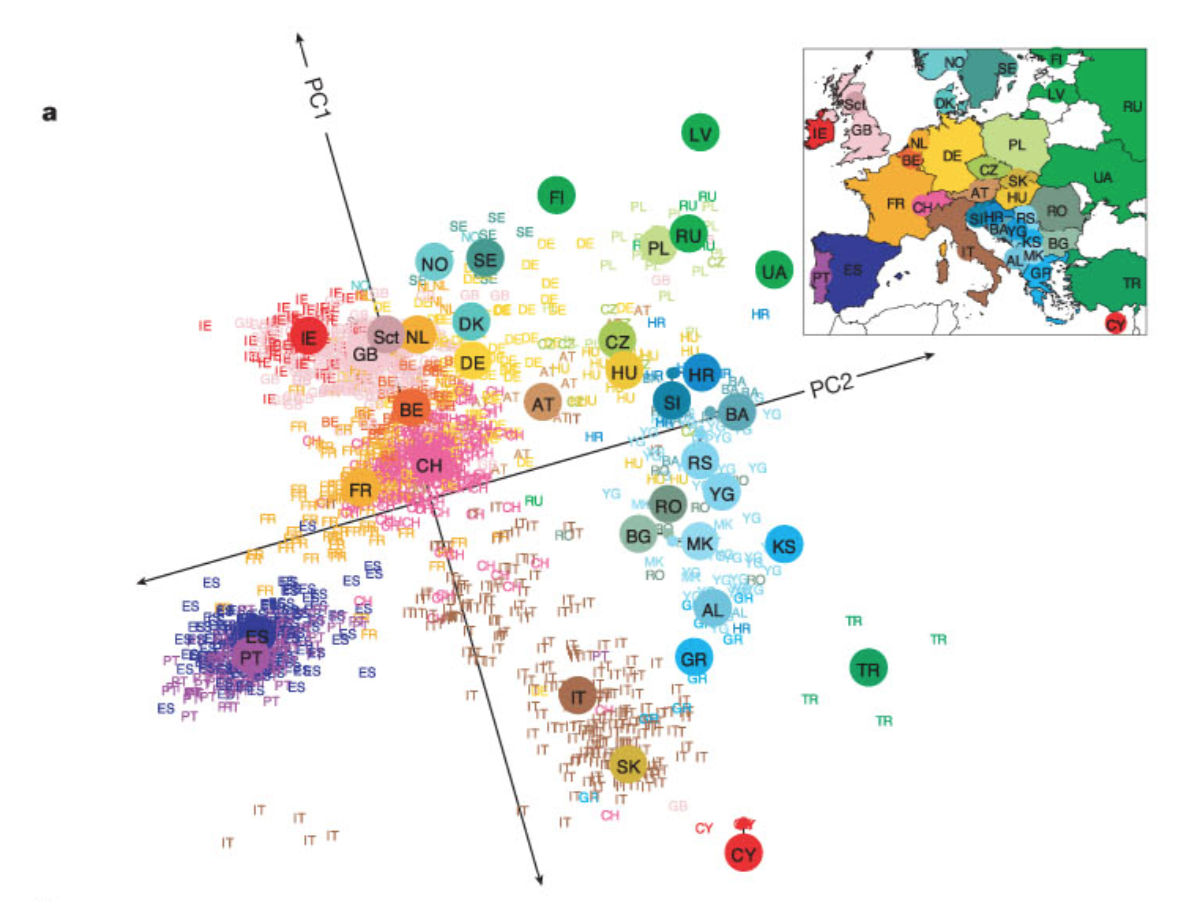
\includegraphics[width=.8\textwidth]{images_20171102_gg04.png}
\end{center}
\end{frame}

%------------------------------------------------
\begin{frame}
\frametitle{Mouse Lemurs}
\begin{center}
		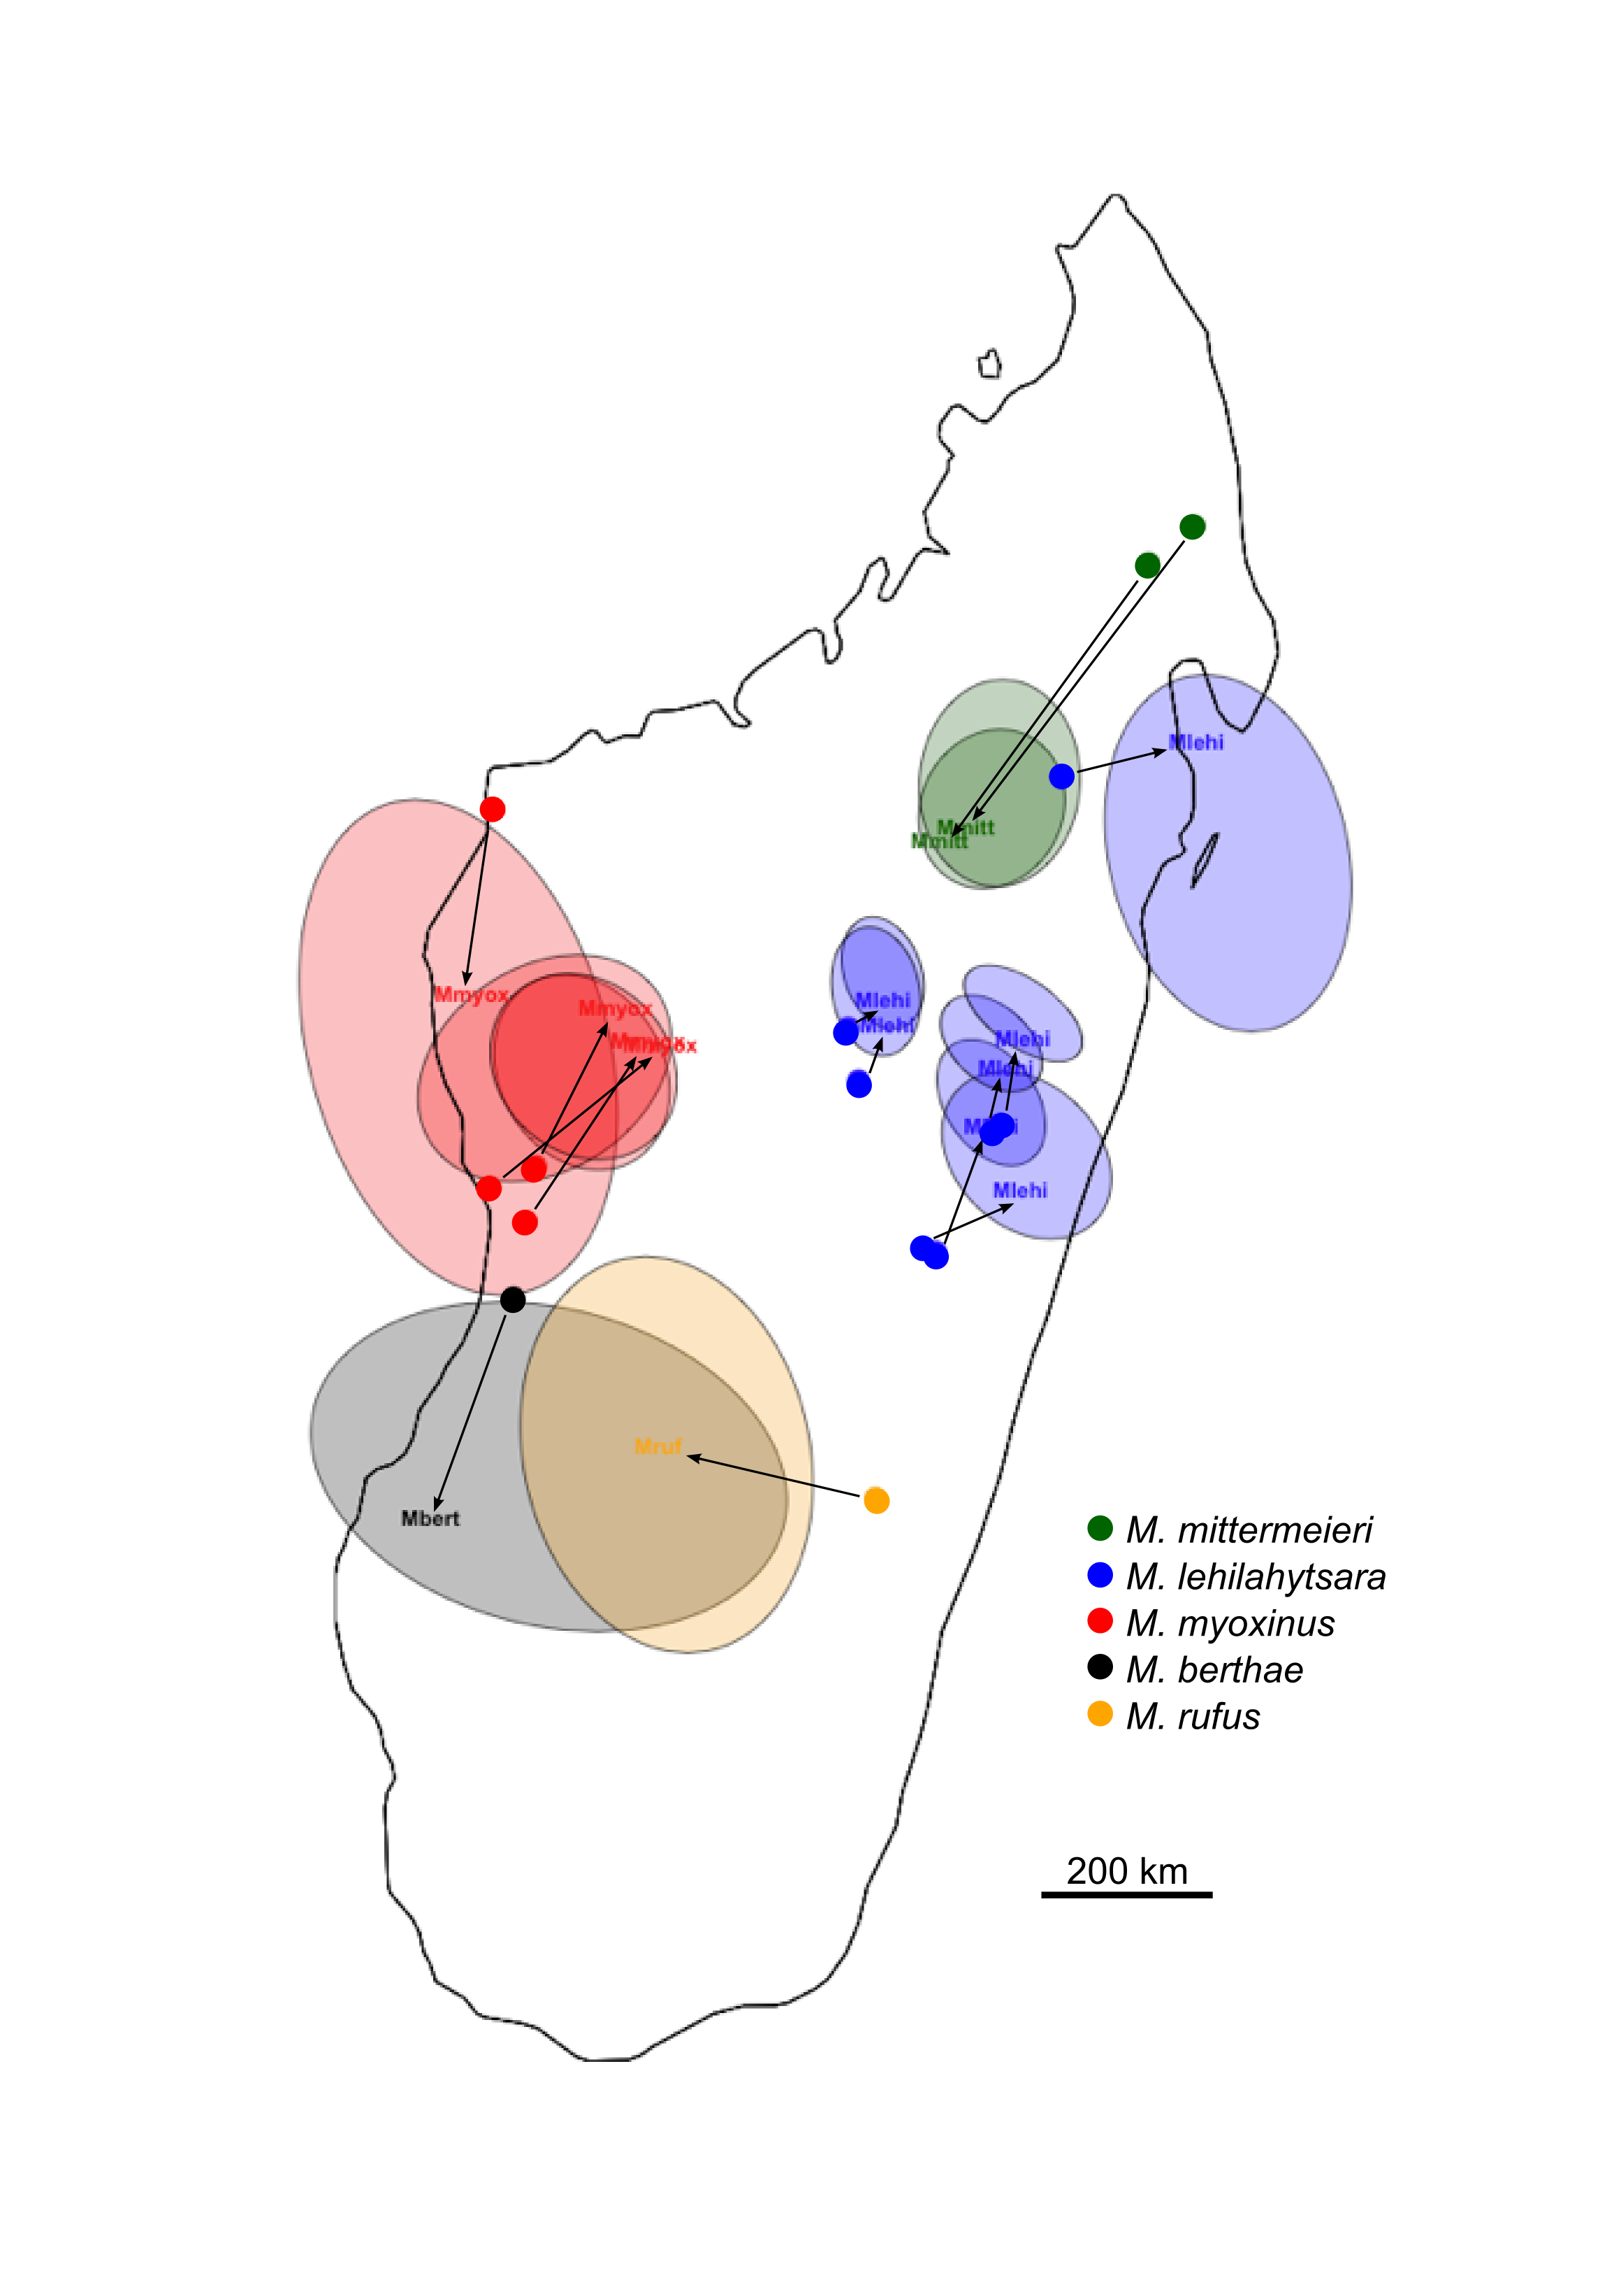
\includegraphics[width=.5\textwidth]{images_20171102_gg05.png}
\end{center}
\end{frame}



%------------------------------------------------
\begin{frame}
\frametitle{Novembre Talk}
\begin{itemize}
	\item[] UPGG Distinguished Lecturer Series
	\item[] John Novembre, University of Chicago
	\item[] "New lenses on human genetic variation: Tools for interpreting geographic structure in genetic data"
	\item[] 4:00pm, 103 Bryan Research Auditorium
\end{itemize}
\end{frame}


%------------------------------------------------
\section{Workflow}
%------------------------------------------------

%------------------------------------------------
\begin{frame}
\frametitle{SLURM Interactive Node}
\begin{itemize}
	\item Later we'll be troubleshooting \texttt{htseq-count}
	\item For that you should use an ``interactive node''
	\item This runs like a sbatch job, but it appears as a terminal that you can interact with
	\footnotesize
	\ttfamily
	\begin{block}{}
	\item[] srun --mem-per-cpu=4000MB --pty bash -i
	\end{block}
	\sffamily
	\item You've just requested a 4GB (powerful laptop) size node on SLURM
\end{itemize}
\end{frame}


%------------------------------------------------
\section{Alignment}
%------------------------------------------------

%------------------------------------------------
\subsection{tophat}
%------------------------------------------------

%------------------------------------------------
\begin{frame}
\frametitle{tophat}
\begin{itemize}
	\item<+-> tophat2 - alignment software
	\item<+-> In: Sequence data
	\item<+-> Out: .bam file - where that data aligns to/fits in the genome
\end{itemize}
\end{frame}

%------------------------------------------------
\begin{frame}
\frametitle{tophat}
\begin{itemize}
	\item tophat2 is the command/software that aligns the reads to the genome
	\item This (also) is going to be a computationally intensive process
	\item So write a submission script to do it:
	\footnotesize
	\ttfamily
	\begin{block}{}
	\item[] export PATH=/opt/apps/tophat-bowtie/:\$PATH
	\item[]
	\item[] tophat2
	\end{block}
	\sffamily
\end{itemize}
\end{frame}

%------------------------------------------------
\begin{frame}
\frametitle{tophat}
\begin{itemize}
	\item tophat2 example (all one line):
	\footnotesize
	\ttfamily
	\begin{block}{}
	\item[]  tophat2 -p 4 -o s01 -G /work/cc216/490S/cc216/RNAseq\_pt2/hsap\_annotations.gff /work/cc216/490S/cc216/RNAseqpt2/hsap /work/cc216/490S/cc216/RNAseq\_pt2/s01\_hsap\_norm\_R1.fastq /work/cc216/490S/cc216/RNAseq\_pt2/s01\_hsap\_norm\_R2.fastq
	\item[] 
	\end{block}
	\sffamily
	\item[] translated:
	\ttfamily
	\begin{block}{}
	\item[]  tophat2 -p <number of threads> -o <output dir> -G <gff file, annotations> <bowtie2 index> <R1 fastq> <R2 fastq>
	\item[] 
	\end{block}
	\sffamily
	\item Help can be found by running ``tophat2''
	\item Or in the tophat2 manual online
	\item \href{http://ccb.jhu.edu/software/tophat/manual.shtml}{http://ccb.jhu.edu/software/tophat/manual.shtml}
\end{itemize}
\end{frame}

%------------------------------------------------
\section{Counting}
%------------------------------------------------

%------------------------------------------------
\begin{frame}
\frametitle{Counting \& Analysis}
\begin{itemize}
	\item<+-> Now that we have bam files the next step is to count the reads
	\item<+-> And using those counts compare gene expression levels
	\item<+-> We'll be using HTseq
\end{itemize}
\end{frame}

%------------------------------------------------
\begin{frame}
\frametitle{HTSeq}
\begin{itemize}
	\item<+-> python-based program to count reads
	\item<+-> Input: 
	\item<+-> .bam file \underline{and} .gtf/.gff
	\item<+-> Output:
	\item<+-> A table of counts by gene
\end{itemize}
\end{frame}

%------------------------------------------------
\begin{frame}
\frametitle{htseq-count}
\begin{itemize}
	\item We'll be using htseq-count
	\item This will count the number of reads mapped to each gene
	\item That data will be taken into DESeq2
	\footnotesize
	\ttfamily
	\begin{block}{}
	\item[] /opt/apps/rhel7/Python-2.7.11/bin/htseq-count 
	\end{block}
	\sffamily
	\item[] (go ahead and put it in your path)
\end{itemize}
\end{frame}

%------------------------------------------------
\begin{frame}
\frametitle{htseq-count}
\begin{itemize}
	\item What does HTSeq do?
	\item What are its flags and options?
	\footnotesize
	\ttfamily
	\begin{block}{}
	\item[] htseq-count <options> <alignment bam> <gff file>  >  <count output>
	\end{block}
	\sffamily
	\item Probably important: -f, -s, -t
\end{itemize}
\end{frame}

%------------------------------------------------
\section{Tutorial Files}
%------------------------------------------------

%------------------------------------------------
\begin{frame}
\frametitle{Files to Use}
\begin{itemize}
	\item I've set up some example files to use for this tutorial
	\item They're human RNAseq files from a hypoxia experiment:
	\footnotesize
	\ttfamily
	\begin{block}{}
	\item[] ls -lthr /work/cc216/490S/cc216/RNAseq\_pt2
	\end{block}
	\sffamily
\end{itemize}
\end{frame}

%------------------------------------------------
\subsection{Commands}
%------------------------------------------------

%------------------------------------------------
\begin{frame}
\frametitle{SLURM Interactive Node}
\begin{itemize}
	\item Now that we're about to troubleshoot \texttt{htseq-count} hopefully your SLURM node is open
	\footnotesize
	\ttfamily
	\begin{block}{}
	\item[] srun --mem-per-cpu=4000MB --pty bash -i
	\end{block}
	\sffamily
\end{itemize}
\end{frame}

%------------------------------------------------
\begin{frame}
\frametitle{tophat}
\begin{itemize}
	\item tophat2 example (all one line):
	\footnotesize
	\ttfamily
	\begin{block}{}
	\item[]  tophat2 -p 4 -o s01 -G /work/cc216/490S/cc216/RNAseq\_pt2/hsap\_annotations.gff /work/cc216/490S/cc216/RNAseqpt2/hsap /work/cc216/490S/cc216/RNAseq\_pt2/s01\_hsap\_norm\_R1.fastq /work/cc216/490S/cc216/RNAseq\_pt2/s01\_hsap\_norm\_R2.fastq
	\item[] 
	\end{block}
	\sffamily
	\item[] translated:
	\ttfamily
	\begin{block}{}
	\item[]  tophat2 -p <number of threads> -o <output dir> -G <gff file, annotations> <bowtie2 index> <R1 fastq> <R2 fastq>
	\item[] 
	\end{block}
	\sffamily
	\item Help can be found by running ``tophat2''
	\item Or in the tophat2 manual online
	\item \href{http://ccb.jhu.edu/software/tophat/manual.shtml}{http://ccb.jhu.edu/software/tophat/manual.shtml}
\end{itemize}
\end{frame}

%------------------------------------------------
\begin{frame}
\frametitle{htseq-count}
\begin{itemize}
	\item What does HTSeq do?
	\item What are its flags and options?
	\footnotesize
	\ttfamily
	\begin{block}{}
	\item[] htseq-count <options> <alignment bam> <gff file> > <count output>
	\end{block}
	\sffamily
	\item Probably important: -f, -s, -t
\end{itemize}
\end{frame}

%------------------------------------------------
\begin{frame}
\frametitle{Today's Goals}
\large
\begin{enumerate}
	\item<+-> Logon to interactive SLURM node
	\item<+-> Run tophat2
	\item<+-> Run htseq-count
\end{enumerate}
\end{frame}

%------------------------------------------------
\subsection{DESeq2}
%------------------------------------------------

%------------------------------------------------
\begin{frame}
\frametitle{DESeq2}
\begin{itemize}
	\item<+-> What does DESeq2 do?
	\item<+-> Compares the count matrices from many samples
	\item<+-> Where do you run it?
	\item<+-> In R on your laptop
\end{itemize}
\end{frame}

%------------------------------------------------
\begin{frame}
\frametitle{DESeq2}
\begin{itemize}
	\item<+-> R-based program to analyze expression
	\item<+-> Input: 
	\item<+-> A table of counts by gene
	\item<+-> Output: 
	\item<+-> Graphs and (hopefully) Answers!!!
\end{itemize}
\end{frame}


%------------------------------------------------
\begin{frame}
\frametitle{DESeq2 guides}
\begin{itemize}
	\item We'll get into DESeq2 next week
	\item If you want to get started here are some guides:
	\item \href{http://bioconductor.org/packages/devel/bioc/vignettes/DESeq2/inst/doc/DESeq2.html}{Walkthrough Link}
	\item Focus on ``Quick Start'' and more specifically:
	\item Setting the R objects \texttt{cts} and \texttt{coldata} correctly
	\item Using \texttt{paste} (a unix command) to format your data into \texttt{cts}
	\footnotesize
	\item[] http://bioconductor.org/packages/devel/bioc/vignettes/
	\item[] DESeq2/inst/doc/DESeq2.html
\end{itemize}
\end{frame}


%------------------------------------------------
\begin{frame}
\Huge{\centerline{The End}}
\end{frame}

%----------------------------------------------------------------------------------------

\end{document} 